\documentclass[11pt]{article}
\usepackage[margin=1in]{geometry}
\usepackage{graphicx}
\usepackage{booktabs}
\usepackage{amsmath}
\usepackage[hidelinks]{hyperref}
\usepackage{caption}
\captionsetup{font=small,labelfont=bf}
\setlength{\parskip}{4pt}

\title{\textbf{An independently detected and vetted 5.45-day, Earth-sized transit candidate in the TOI-913 system (TIC 407126408)}}
\author{Josh Gold\\ \small Independent researcher, Acton, Massachusetts, USA}
\date{\small Preprint, version 2, 12 October 2026 (version 1: 11 October 2026). Not peer reviewed.\\ Version 1 DOI: \href{https://doi.org/10.5281/zenodo.23290579}{10.5281/zenodo.23290579}}

\begin{document}
\maketitle

\begin{abstract}
\noindent We report a transit-like signal with period $P = 5.450138 \pm 0.000016$\,d and depth $196^{+24}_{-21}$\,ppm on the K dwarf TOI-913 (TIC 407126408; $V=10.5$, $d=65.2$\,pc), which hosts the confirmed sub-Neptune TOI-913\,b ($P = 11.0994$\,d). The signal was found by an automated multi-sector search of TESS 2-minute photometry spanning Sectors 12--102 (2019--2026; 34 transits) and corresponds to a radius of $1.12 \pm 0.09\,R_\oplus$ if it arises on the target. It passes ten automated false-positive tests, including odd/even depth, secondary eclipse, shape, per-sector consistency and a season-holdout prediction test. It is independently recovered as the strongest periodic signal in Quick-Look Pipeline full-frame-image photometry. In 200 block-shuffled copies of the light curve, no transit search reached the observed signal strength (empirical false-alarm probability $<1.5\%$ at 95\% confidence), although this test does not capture systematics coherent over many days. In the inverted light curve, which keeps such systematics, the strongest peak unrelated to TOI-913\,b reaches SDE 14.5, against 21.7 for the signal. A transit fit with free stellar density yields $\rho_\star = 2.43^{+0.96}_{-1.02}\,\rho_\odot$, consistent with the catalogue value $2.09 \pm 0.45\,\rho_\odot$. The only Gaia neighbour previously flagged as able to produce the depth, TIC 407126405 at $9.5''$, is a background giant ($R\approx10\,R_\odot$, $d\approx5$\,kpc) whose geometry cannot reproduce the observed 2.4\,h duration. TESS difference-image centroids cannot separate it from the target, so this exclusion rests on the duration alone. With archival Gemini/Zorro speckle constraints, and with a catalogue entry at $56.9''$ removed because it is a galaxy rather than a star, \textsc{TRICERATOPS} gives FPP $=0.036$ and NFPP $=0.023$, which meets neither the ``validated'' nor the ``likely planet'' criteria of Giacalone et al.\ (both require NFPP $<0.001$). The residual nearby-eclipsing-binary probability comes mostly from two faint stars at $26.5''$ and $58.0''$; per-sector centroids from an independent pipeline disfavour the first. Seeing-limited ground-based photometry could test both. A 27.3\,d systematic in the light curve lies near five times the period, but the two drift apart by 0.59 of a period over the baseline, and the transits far from any 27.3\,d event carry the full depth, so the signal is not a harmonic of it. The signal was also detected by the independent open-source search \texttt{eumemic/exoplanets} (2026 October 8), which set it aside because of the $9.5''$ neighbour, and at a detection strength (MES 8.0--9.6) below that search's candidate threshold of MES 10, where it finds a third to a half of signals to be false alarms. We present it as a planet candidate, not a confirmed planet. If real, it lies near the 2:1 period commensurability with TOI-913\,b ($P_b/P_c = 2.037$).
\end{abstract}

\section{Introduction}
Faint transit signals from small planets can become detectable only once several years of TESS photometry are combined. This project was inspired by the approach of P.~Rabtsevich \cite{rabtsevich}, who stacked TESS sectors from several years for a single star and then tried systematically to falsify the resulting candidate, including by hiding one observing season and predicting its transit times. We automated that approach for a sample of nearby K and M dwarfs. In a 200-star pilot, one previously unreported signal survived all automated tests. This note documents that signal and our attempts to rule it out.

TOI-913 (TIC 407126408) is a K dwarf ($T_\mathrm{eff}=4969$\,K, $R_\star = 0.733\,R_\odot$, $M_\star = 0.82\,M_\odot$; TIC 8 \cite{stassun}) at 65.2\,pc (Gaia DR3 parallax $15.31\pm0.02$\,mas \cite{gaia}). It hosts TOI-913\,b, a $2.45\,R_\oplus$ planet at 11.0986\,d, statistically validated by Mistry et al.\ \cite{mistry}, and the long-period candidate TOI-913.02, seen in two transits.

\section{Data and search}
We used SPOC \cite{jenkins} PDCSAP 2-minute light curves for Sectors 12, 13, 65, 66, 93, 100, 101 and 102, retrieved with \texttt{lightkurve} \cite{lightkurve}. Quality-flagged cadences were removed and only upward outliers were clipped. Each sector was normalized and detrended with a biweight filter (\texttt{wotan} \cite{wotan}) with a 0.61\,d window. We searched with transit least squares (TLS \cite{tls}) over 0.5--40\,d on 10-minute bins, iteratively masking each detection. Detection required SDE $\geq 9$, SNR $\geq 7$ and $\geq 3$ transits. TLS 2.0 multiplies trial durations by a ``fill factor'' (data span over baseline). On multi-year data with large gaps, this shortened durations about $20\times$ and suppressed SNR about $4\times$, so we disabled it.

After TOI-913\,b (SDE 125.5, SNR 34.3), the search found a 27.3\,d systematic, which the kill tests rejected, and then the 5.45\,d signal (SDE 23.6, SNR 8.9, 34 transits). The 5.45\,d signal is therefore not the strongest peak in the search until that systematic is masked; in an unmasked search of the standard light curve it ranks sixth (Table~\ref{tab:rob}). Before the kill tests, the light curve was re-detrended with all detected transits masked.

\paragraph{Pipeline validation.} Before the pilot, the pipeline was run on 20 hosts of 26 confirmed small planets and on 10 detached eclipsing binaries from the TESS EB catalogue \cite{prsa}. It recovered 23/26 planets at the correct period, and all 23 survived every hard test. The three misses had only 1--2 sectors. It rejected 8/9 detected binaries; the exception is a twin-eclipse binary detected at half its period. In an injection-recovery grid on two quiet stars, planets $\geq1.5\,R_\oplus$ were recovered out to 15\,d, and planets $\geq2\,R_\oplus$ out to 30\,d.

\section{The signal}
Figure~\ref{fig:fold} shows the folded transit. We fit both planets jointly with \texttt{batman} \cite{batman} and \texttt{emcee} \cite{emcee}. Each planet had a free period, epoch, $R_p/R_\star$ and impact parameter, on circular orbits, with quadratic limb darkening fixed to $(0.451, 0.189)$ and a jitter term. We ran two fits: one with a shared stellar density and a catalogue prior, and one with an independent density per planet and no prior. Table~\ref{tab:params} lists the results.

\begin{figure}[!htbp]
\centering
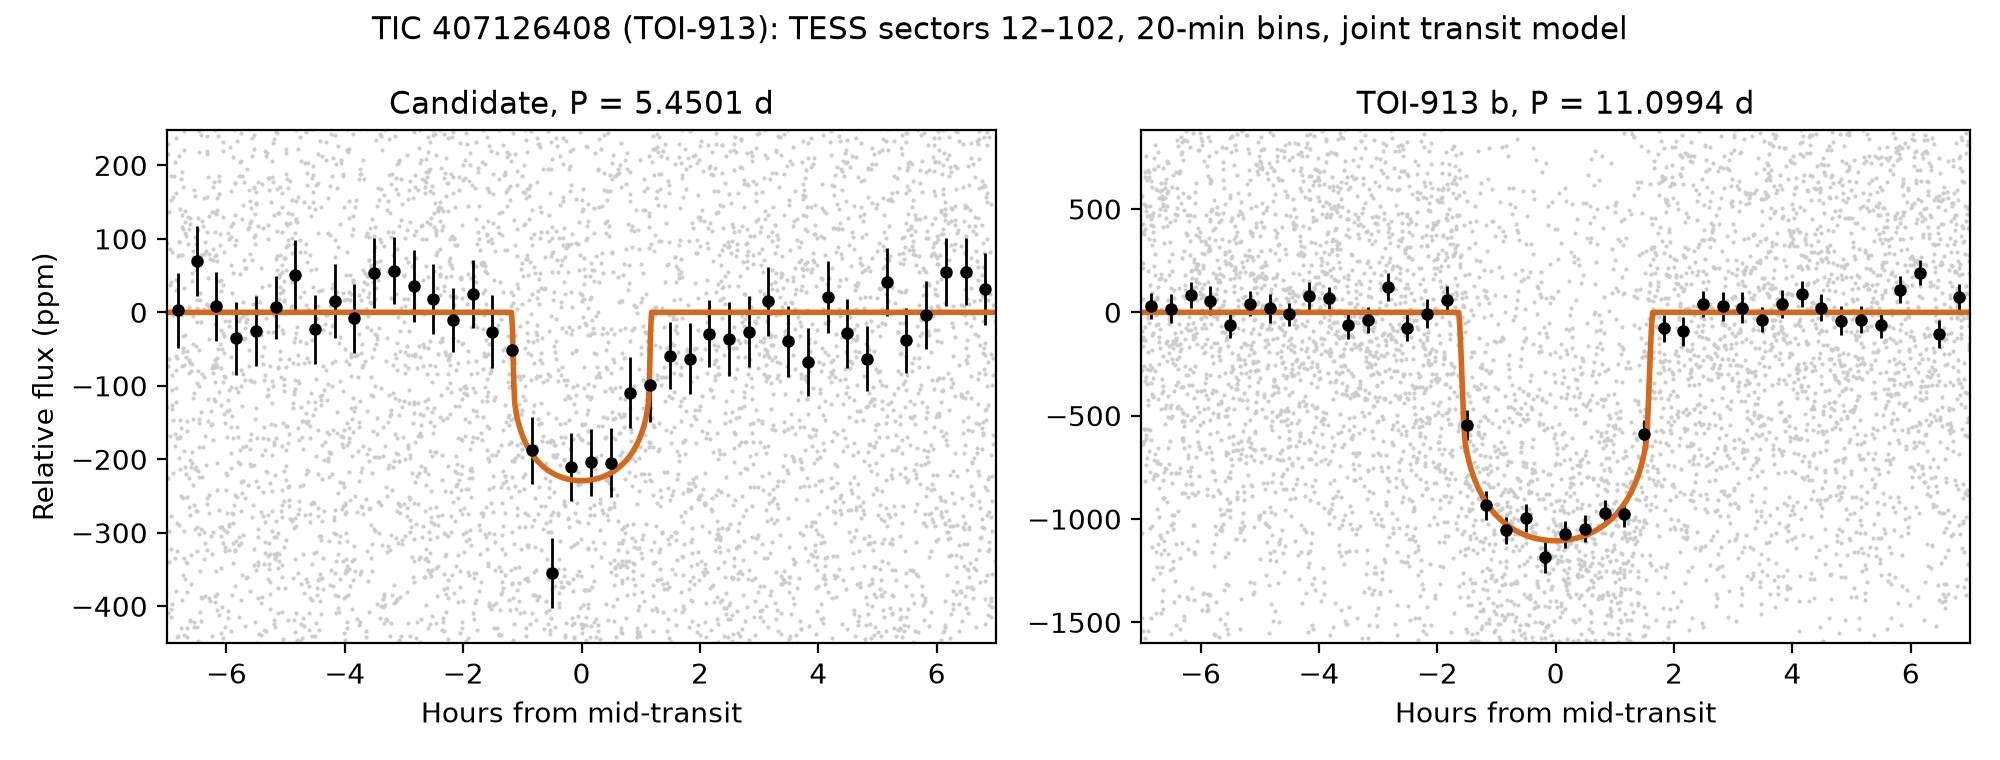
\includegraphics[width=\textwidth]{figures/fig1_fold.png}
\caption{Phase-folded TESS photometry of TOI-913 (Sectors 12--102) at the candidate period (left) and at TOI-913\,b's period (right), each with the other planet's model removed. Grey: 2-minute data; black: 20-minute bins; orange: joint transit model.}
\label{fig:fold}
\end{figure}

\begin{table}[h]
\centering
\small
\begin{tabular}{lcc}
\toprule
Parameter & Candidate (``.03'') & TOI-913\,b \\
\midrule
Period (d) & $5.450138 \pm 0.000016$ & $11.09938$ (fit) \\
$T_0$ (BJD$_\mathrm{TDB}$) & $2458628.6479^{+0.0046}_{-0.0073}$ & --- \\
Depth (ppm) & $196^{+24}_{-21}$ & $912^{+27}_{-24}$ \\
$R_p/R_\star$ & $0.0140 \pm 0.0008$ & --- \\
$R_p$ ($R_\oplus$) & $1.12 \pm 0.09$ & $2.4$ \\
Impact parameter & $0.42^{+0.13}_{-0.21}$ & $0.19^{+0.16}_{-0.13}$ \\
$T_{14}$ (h) & $2.37^{+0.16}_{-0.15}$ & $3.27$ \\
$\rho_\star$, free fit ($\rho_\odot$) & $2.43^{+0.96}_{-1.02}$ & $1.61^{+0.40}_{-0.75}$ \\
$a$ (AU), $T_\mathrm{eq}$ (K, $A=0$) & $0.057$, $\sim860$ & $0.091$, $\sim680$ \\
\bottomrule
\end{tabular}
\caption{Transit parameters. The joint fit has a shared density with a catalogue prior of $2.09\pm0.45\,\rho_\odot$; the free fit has no prior. The $R_p$ uncertainty includes a 5\% uncertainty on $R_\star$.}
\label{tab:params}
\end{table}

\section{Vetting}
\subsection{Automated tests}
The signal passed all hard tests: odd/even depth ($211$ vs $245$\,ppm, $0.4\sigma$); secondary eclipse at phase 0.5 and across phases 0.3--0.7 (maximum $2.4\sigma$); duration plausibility; size; per-sector depth consistency ($p=0.17$); harmonic relation to TOI-913\,b ($P_b/P = 2.037$, not an integer ratio); and an injection test at the same period and depth. The trapezoid shape test was inconclusive at this SNR. In a season-holdout test, each of the four observing seasons was hidden, the ephemeris was fitted on the rest, and depth was measured only at the predicted times. Three of four seasons showed the transit at $>2\sigma$. The fourth (Sector 93 alone) gave $1.8\sigma$. Figure~\ref{fig:diag} shows the diagnostic page. A fresh, read-only AI review of that page flagged the $9.5''$ neighbour and the depth scatter between sectors, both addressed below.

\begin{figure}[!htbp]
\centering
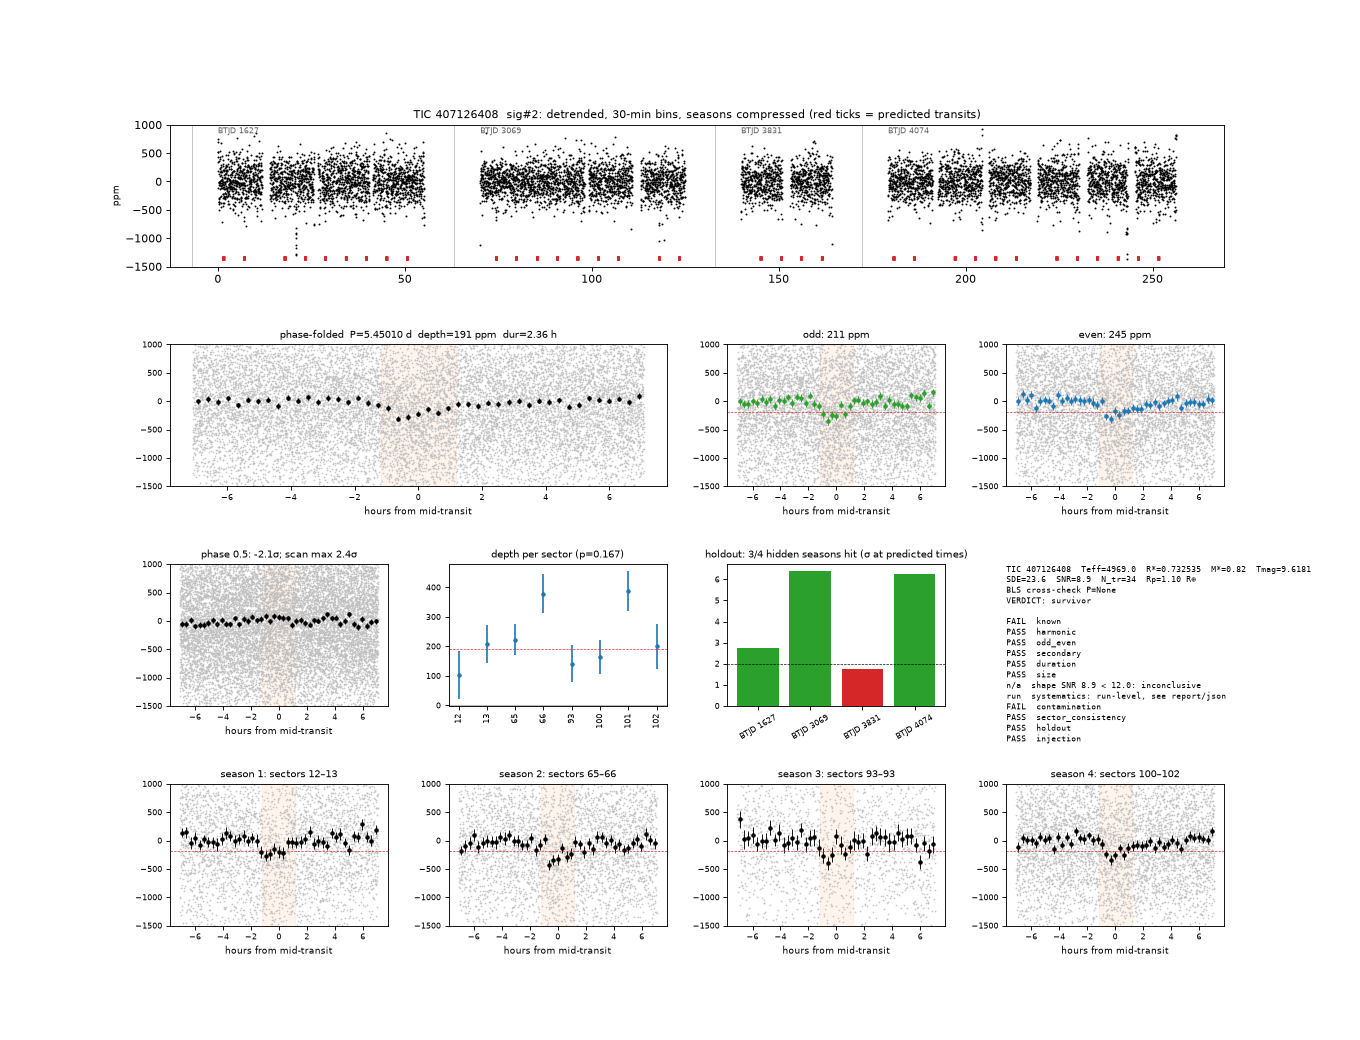
\includegraphics[width=\textwidth]{figures/fig2_diagnostic.png}
\caption{Pipeline diagnostic page: full light curve with predicted transits (red), fold, odd/even, phase 0.5, depth per sector, the holdout test, and folds per season.}
\label{fig:diag}
\end{figure}

\subsection{Robustness}
We remeasured the depth over the central 60\% of the transit, with red-noise-aware errors, across variants (Table~\ref{tab:rob}). Every season and sector jackknife gives 196--244\,ppm. No transit departs by $>3\sigma$ from the mean, and removing the three deepest leaves $190\pm25$\,ppm. One of 34 transits lies within 0.5\,d of a data gap (8\% expected by chance), and none lie within 0.1\,d of a momentum dump (43 dump events, comprising 231 flagged cadences; version 1 called these ``231 momentum dumps''). The only non-confirming variant is uncorrected SAP flux. There the signal is weaker ($159\pm24$\,ppm, SNR 6.6) and a narrow search drifts to 5.427\,d.

\begin{table}[h]
\centering
\footnotesize
\begin{tabular}{lccl}
\toprule
Variant & Depth (ppm) & SNR & Full 0.5--40\,d TLS search \\
\midrule
PDCSAP, biweight 0.61\,d & $225 \pm 24$ & 9.5 & rank 6 (systematics unmasked) \\
Biweight 0.5 / 0.75 / 1.0 / 1.5\,d & 230 / 232 / 231 / 235 & 9.0--9.9 & --- \\
Cosine detrending & $297 \pm 23$ & 13.1 & \textbf{5.4501\,d top peak} (SDE 12.8) \\
QLP FFI photometry (8 sectors) & $250 \pm 23$ & 10.6 & \textbf{5.4501\,d top peak} (SDE 15.2) \\
TESS-SPOC FFI & $185 \pm 31$ & 6.0 & --- \\
SAP flux (uncorrected) & $159 \pm 24$ & 6.6 & not recovered \\
\bottomrule
\end{tabular}
\caption{Signal depth across data products and detrending choices, with TOI-913\,b and TOI-913.02 masked.}
\label{tab:rob}
\end{table}

\subsection{Is the signal on the target?}
\textbf{Stellar density.} With no prior, the transit shape implies $\rho_\star = 2.43^{+0.96}_{-1.02}\,\rho_\odot$. That agrees with the TIC value ($2.09\pm0.45$) and with the density from TOI-913\,b's transit.

\textbf{The $9.5''$ neighbour.} TIC 407126405 ($T=14.05$, $\Delta T = 4.4$) lies within one TESS pixel. It is a background giant: Gaia parallax $0.16\pm0.02$\,mas, TIC $R = 10.0\,R_\odot$, luminosity class giant. To produce the observed dilution it would need a $\approx1.1\%$ eclipse. An orbit with $P=5.45$\,d around a $10\,R_\odot$, 1--3\,$M_\odot$ star has $a/R_\star \approx 1.4$--$1.9$, so a central transit lasts $\approx23$--33\,h. A grazing chord short enough to last 2.4\,h would occult at most $\sim$0.02\% of the stellar disk. We therefore exclude this star as the source. \textsc{TRICERATOPS} assigns it negligible probability ($\sim10^{-26}$), but this follows from the same catalogue radius and is not independent evidence. No pixel-level test separates the two stars (below), so the exclusion rests on the duration argument and the TIC radius.

\textbf{Pixel-level tests.} We stacked per-sector difference images and compared fits with the source at the target or at a neighbour (Figure~\ref{fig:pix}). For the $9.5''$ star, the test has little power at this SNR. A control on TOI-913\,b prefers the target at only $\approx2\sigma$, and the candidate gives no preference ($0.5\sigma$). It is likewise inconclusive for the two faint neighbours below ($0.8\sigma$ and $0.2\sigma$). In one sector (S65), the fit prefers the $56.9''$ source at $\approx3\sigma$, but this is not significant over all sectors, and that source is a galaxy (Section~4.5). We report these as non-constraining.

\textbf{Independent centroids.} The \texttt{eumemic/exoplanets} team fitted PRF centroids to difference images in all eight sectors \cite{eumemicissue}. Per-sector offsets from the target range from $0.4''$ to $26.8''$, and the quality-weighted mean lies about $5''$ from the target, toward TIC 407126405. They therefore do not separate the target from the $9.5''$ giant, and we do not use them for that purpose. (An earlier statement of a $0.36''$ offset referred to the best single sector and was withdrawn by that team.) They do argue against TIC 407126406, the star that dominates the NFPP, and against the $56.9''$ source: no sector places the centroid within $11''$ of TIC 407126406 or within $30''$ of TIC 10001766874. In that team's calibration on known TOIs, signals from stars 21--$63''$ away produced offsets above $15''$ in 98--100\% of cases. This does not cover TIC 407126397, and it is TESS-pixel evidence, not a substitute for ground-based photometry.

\begin{figure}[!htbp]
\centering
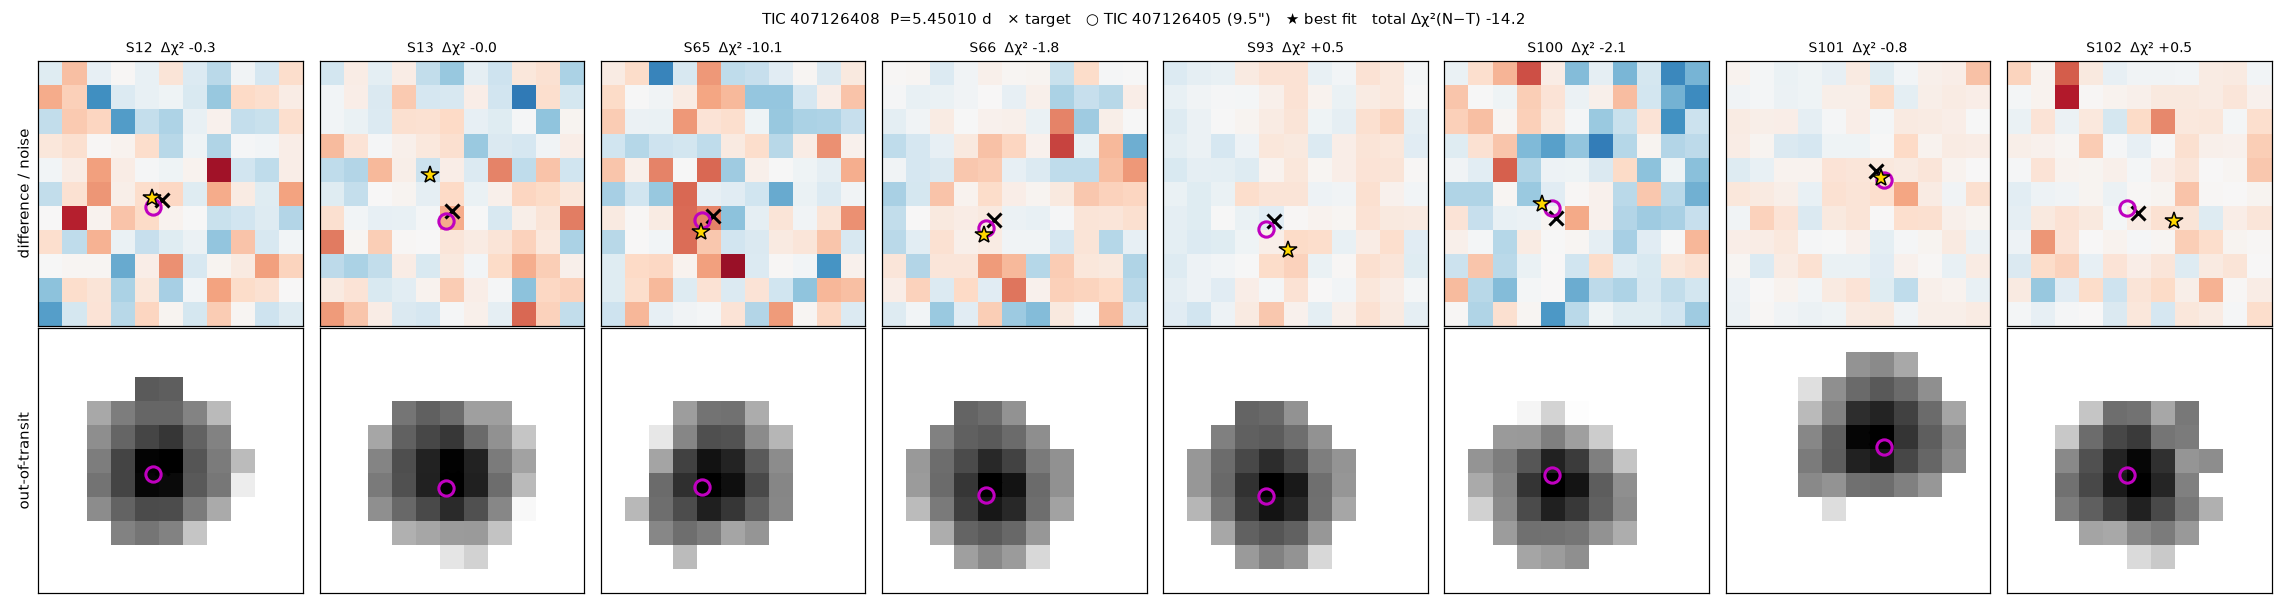
\includegraphics[width=\textwidth]{figures/fig3_pixel_giant.png}
\caption{Per-sector difference images (top: lost flux over noise) and out-of-transit images (bottom). $\times$: target; $\circ$: TIC 407126405; $\star$: best-fit location. TESS's $21''$ pixels cannot separate the $9.5''$ pair at this SNR.}
\label{fig:pix}
\end{figure}

\textbf{High-resolution imaging.} Archival speckle imaging on ExoFOP shows no companions to contrasts of $\Delta m = 6.47$ at $0.5''$ (Gemini/Zorro, 832\,nm, 2020 March 14) and $\Delta m = 6.9$ at $1''$ (SOAR/HRCam, $I$, 2019 August 12).

\subsection{Periodograms and empirical false-alarm probability}
The search threshold (SDE $\geq9$) is calibrated on white noise, so we measured the false-alarm probability on this star's own light curve (Figure~\ref{fig:pgram}; code \texttt{periodogram\_fap.py}). All tests use the light curve of Section~2.

\textbf{Matched-filter test.} We reran the same TLS search on 200 copies of the light curve in which 1-day blocks were shuffled within each sector. This keeps noise on timescales below a day and destroys any coherent period. Each copy used the masks in place when the pipeline found the signal (TOI-913\,b, the two TOI-913.02 events and the 27.3\,d systematic). On the real data, 5.4501\,d is the top peak, at SDE 21.8. The highest SDE anywhere in 0.5--40\,d across the shuffled copies had a median of 13.1, a 99th percentile of 18.1 and a maximum of 18.8. None reached 21.8, so the false-alarm probability is $<1.5\%$ (95\% upper limit). Block shuffling does not reproduce systematics coherent over many days, such as the 27.3\,d signal that outranks the candidate in the unmasked search, so the true false-alarm probability may be higher than this test indicates. For comparison, the \texttt{eumemic/exoplanets} search of inverted light curves finds that $37\pm4\%$ of vetted signals at MES 9--10 are false alarms, averaged over $\sim8\times10^5$ stars \cite{eumemicissue}.

\textbf{Inverted light curve.} To test systematics that last longer than a day, we followed a suggestion from \texttt{eumemic/exoplanets} \cite{eumemicissue} and ran the same TLS search, with the same masks, on the light curve reflected about its median (code \texttt{inversion\_test.py}). Inversion keeps the timing and timescale of every systematic but turns dips into bumps, so the strongest inverted peak shows how strong a signal this light curve's systematics alone can produce. The flux was inverted after normalisation and before outlier clipping and detrending, so the inverted copy went through the same preparation as the real one. Each search was repeated four times, masking the top peak each time. The two strongest inverted peaks (SDE 18.2 and 15.6) lie at TOI-913\,b's period, 11.10\,d, with epochs 0.18\,d before and 0.21\,d after b's transits, just outside its mask. They are the shoulders the biweight filter leaves beside a transit it did not mask, not a property of the star's light curve. The strongest inverted peak unrelated to b is at 38.8\,d (SDE 14.5, three transits). The candidate, at SDE 21.7 in the same run, exceeds both. This is a single inverted copy, so it gives a comparison rather than a probability. It agrees with the shuffled test, and in both cases the noise ceiling sits near SDE 15--19, below the candidate.

\textbf{Harmonic of the 27.3\,d systematic.} The systematic the pipeline rejected at $P_s=27.2852$\,d (five events, $555\pm61$\,ppm) lies close to five times the candidate's period, and a periodic systematic can produce transit-search peaks at $P_s/n$. Here $5P = 27.2507\pm0.0001$\,d, so over the 2524\,d baseline the 5:1 alignment slips by 3.2\,d, 0.59 of the candidate's period, and a harmonic could not stay in phase. We measured the central depth of each transit (the middle 60\% of the transit, against the flux one to three durations either side, at the fitted epoch), which is deeper than the fitted mean depth because of limb darkening. Of the 34 observed transits, the 32 that lie more than 1.4\,d from any 27.3\,d event give a combined central depth of $222\pm22$\,ppm (SNR 10.2), against $227\pm21$\,ppm for all 34. The other two lie 0.41 and 0.44\,d from a 27.3\,d event, outside it, and give $308\pm93$\,ppm. A harmonic would draw its depth only from transits that coincide with the systematic (code \texttt{harmonic\_systematic\_test.py}). The systematic was also masked in the search that found the signal.

\textbf{Generalized Lomb--Scargle.} A GLS periodogram \cite{gls} does not detect the signal: at 5.45\,d the power is $6.0\times10^{-5}$, with Baluev false-alarm probability \cite{baluev} $\approx1$. It does not detect TOI-913\,b either. With b left in the light curve, b's GLS power is $1.8\times10^{-4}$ (rank 1653, false-alarm probability $\approx1$), although TLS detects it at SDE 125. A transit of 2--3\,h fills 1--2\% of the orbit and is poorly matched by a sinusoid. The only GLS peaks above the 0.1\% level lie below 0.8\,d, at the scale of the detrending window. GLS therefore cannot decide this signal either way. In particular, the absence of a GLS peak is not evidence for the signal. It shows only that the light curve has no significant sinusoidal variability at 5.45\,d, such as rotational modulation.

\textbf{Spectral window and momentum dumps.} The window function has power $1.1\times10^{-3}$ at 5.45\,d, against 0.055 at its strongest peak (38\,d). An alias of TOI-913\,b at 5.45\,d would require window power at 10.7\,d, where it is $7\times10^{-4}$. The 43 momentum-dump events are spaced 3.4--6.8\,d apart (median 6.4\,d). In their periodogram, 5.45\,d lies at the 43rd percentile of power. Folded at 5.45\,d, no dump falls in transit (0.8 expected), and their phases show no clustering (Rayleigh $Z=0.04$).

\begin{figure}[!htbp]
\centering
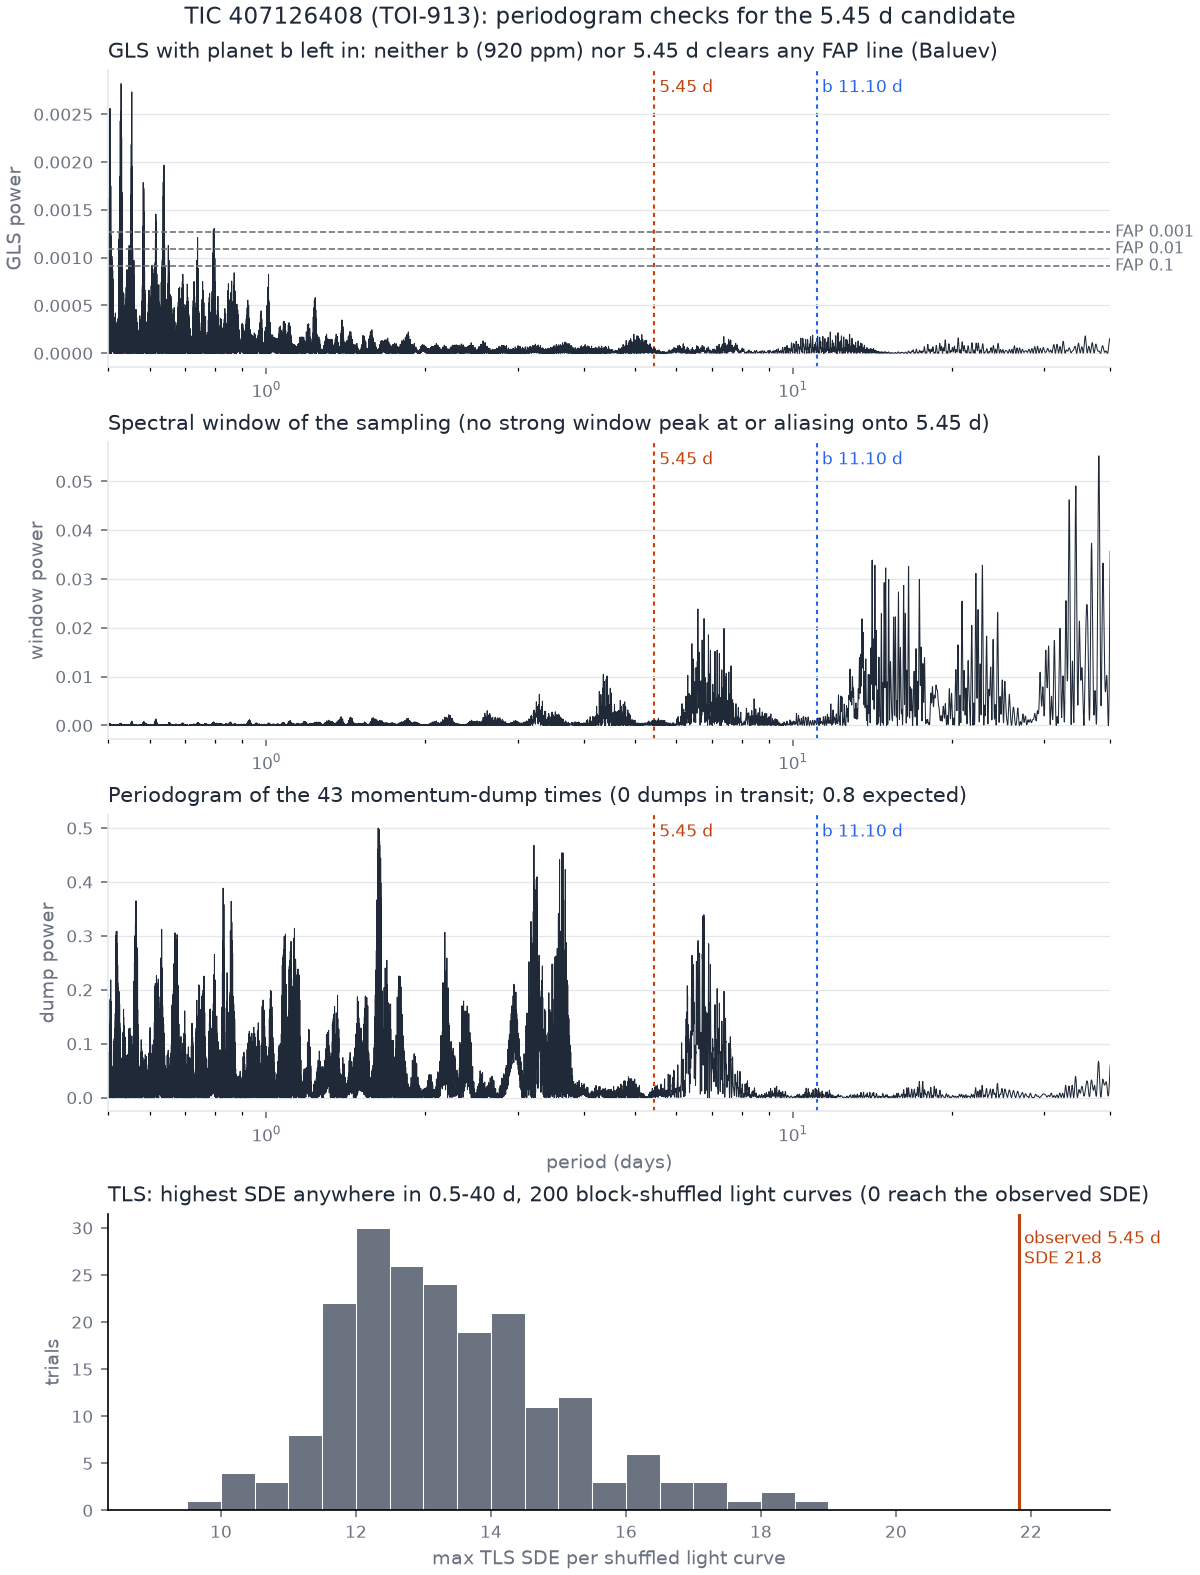
\includegraphics[width=0.85\textwidth]{figures/fig4_periodograms.png}
\caption{From top: GLS periodogram with TOI-913\,b left in, with Baluev false-alarm levels; spectral window; periodogram of the momentum-dump times; and the maximum TLS SDE in each of 200 block-shuffled light curves, against the observed 5.45\,d signal (orange).}
\label{fig:pgram}
\end{figure}

\subsection{False-positive probability}
We ran \textsc{TRICERATOPS} v1.1 \cite{triceratops} on the folded light curve, using the SPOC apertures of all eight sectors and 8 runs of $N=10^6$. Without the contrast curve, FPP $=0.155\pm0.008$ and NFPP $=0.032\pm0.001$. With the Zorro 832\,nm curve, FPP $=0.054\pm0.002$ and NFPP $=0.041\pm0.001$. In that run, NFPP was dominated by NEB scenarios on TIC 10001766874 ($T=15.91$, $56.9''$; would need a 31.7\% eclipse; 0.020), TIC 407126406 ($T=16.97$, $26.5''$; 22.7\%; 0.017) and TIC 407126397 ($T=14.9$, $58.0''$; about 10\%; 0.004).

TIC 10001766874 is not a star. The TIC lists it as an extended source (objType EXTENDED): it is the 2MASS extended source 2MASX J15381760$-$8047167, $12.6''$ across. TIC 407126394, at $57.4''$, is flagged as a duplicate of it, and the only Gaia DR3 source at that position ($G=20.9$) has no parallax or proper motion. It is most likely a galaxy, which cannot host a 32\% eclipse of its total light. We reran \textsc{TRICERATOPS} with the same inputs and both entries removed from the scenarios. They were removed after the flux ratios were computed, so their light still dilutes the aperture (option \texttt{--drop} in \texttt{triceratops\_fpp.py}). This gives FPP $=0.036\pm0.001$ and NFPP $=0.023\pm0.001$, which we adopt. The probability of a planet on the target is 0.94. NFPP now comes from TIC 407126406 (0.018) and TIC 407126397 (0.004); every other star contributes less than 0.001. The no-contrast-curve run above still includes the galaxy. Giacalone et al.\ \cite{triceratops} define a ``validated planet'' as FPP $<0.015$ and NFPP $<0.001$, and a ``likely planet'' as FPP $<0.5$ and NFPP $<0.001$. With NFPP $=0.023$, the candidate meets neither: it is a planet candidate, not a likely or validated planet. (Version 1 said it met the FPP criterion for a likely planet, which was misleading, since that category also requires the NFPP criterion.)

\section{Prior detections}
No CTOI exists for this star on ExoFOP. SPOC multi-sector searches through Sectors 65, 69 and 96 produced TCEs only for TOI-913\,b and TOI-913.02. Scaled to the five sectors available through S96, our signal would have SNR $\approx7.0$, near the SPOC threshold of 7.1. In Sectors 12--13 alone, it has SNR 5.4, which explains its absence from searches limited to early data. The RAVEN FFI survey \cite{raven} (Sectors 1--55) lists a weak second signal on this star at 3.70\,d, which we do not recover in eight sectors (TLS SNR $<6$ near 3.70\,d). The independent open-source search \texttt{eumemic/exoplanets} \cite{eumemic} detected the same signal ($P=5.450121$\,d, 220\,ppm, MES 8.0; MES 9.6 at 5.45017\,d, 224\,ppm in a second search with b masked \cite{eumemicissue}) in its 2026 October 8 release, with the status ``close neighbour could produce the depth''. Our duration argument (Section 4.3) addresses this concern; that team's pipeline requires MES $\geq10$ for candidates. The signal is therefore not in that team's catalogue. In its inverted light curves, about half of the signals below MES 10 are false alarms, and its per-sector centroids cannot distinguish TOI-913 from TIC 407126405 ($p=0.49$ and $0.62$) \cite{eumemicissue}.

\section{Discussion}
If confirmed, the candidate would be a $\sim1.1\,R_\oplus$ planet interior to TOI-913\,b, with $P_b/P_c = 2.037$, just wide of the 2:1 commensurability. For a near-resonant pair, transit-timing variations are expected with a super-period of $|1/P_c - 2/P_b|^{-1}$; this ratio places it near 304\,d. Its mass, with an expected RV semi-amplitude of order 0.5\,m\,s$^{-1}$, is beyond most current spectrographs. The most direct next step is seeing-limited photometry of TIC 407126406 and TIC 407126397 during a predicted transit, to exclude the remaining nearby-eclipsing-binary scenarios. The ephemeris uncertainty in late 2026 is about $\pm15$\,min. The 200\,ppm transit on the target itself is beyond typical ground-based precision, so the strongest test of the signal is TESS Sector 114 (February--March 2027), for which we pre-registered predicted transit times before the data exist \cite{prereg}.

\section{Conclusion}
We present TIC 407126408.03 (proposed designation, pending any CTOI assignment) as a planet candidate. It is a $1.12\pm0.09\,R_\oplus$, 5.450138\,d transit signal that survives automated vetting, independent-product recovery, stellar-density consistency and high-resolution imaging constraints, with FPP $=0.036$ and an empirical false-alarm probability $<1.5\%$ in block-shuffled light curves. No peak in the inverted light curve reaches its strength, and it is not a harmonic of the 27.3\,d systematic. It is not statistically validated, nor a ``likely planet'' (NFPP $=0.023$). Ground-based photometry of two faint neighbours, and the pre-registered TESS Sector 114 transits, are the next tests.

\section*{Acknowledgements}
This work was inspired by P.~Rabtsevich (\href{https://x.com/p_rabtsevich}{@p\_rabtsevich}), who shared his TESS candidate search and methods openly \cite{rabtsevich}. We thank the \texttt{eumemic/exoplanets} project for publishing its independent search openly, and for its all-sector centroid analysis, detection and false-alarm statistics, the suggestion of the inverted-light-curve test, and for pointing out TIC artifact entries among catalogue neighbours. This paper includes data collected by the TESS mission, funded by NASA's Science Mission Directorate, and obtained from MAST at STScI. It uses data and services from ExoFOP-TESS, including high-resolution imaging contributed by S.~Howell (Gemini/Zorro) and A.~Tokovinin (SOAR/HRCam), and data from ESA's Gaia mission. We used QLP and SPOC data products, \texttt{lightkurve}, \texttt{wotan}, \texttt{transitleastsquares}, \texttt{batman}, \texttt{emcee}, \texttt{astropy}, \texttt{astroquery} and \textsc{TRICERATOPS}.

\paragraph{Author and AI assistance.} The author is not a professional astronomer. The search pipeline, the vetting code, the analysis and much of this text were produced with substantial assistance from Anthropic's Claude AI coding agent, directed by the author. Fresh AI sessions were used as adversarial reviewers of diagnostic plots. Every number in this note comes from the released code and data and can be reproduced from them, but no professional astronomer has independently checked the analysis.

\paragraph{Data availability.} Code, per-test result files and figures accompany this preprint in the same Zenodo record, and the code is at \url{https://github.com/killercatfish/tess-hunt}.

\paragraph{Changes from version 1.} Added Section 4.4 (periodograms, empirical false-alarm probability and the inverted-light-curve test) and Figure 4. Corrected the \textsc{TRICERATOPS} classification (Section 4.5): the candidate is not a ``likely planet''. Corrected ``231 momentum dumps'' to 43 dump events (231 flagged cadences). Reported NFPP as $0.041\pm0.001$ (the run mean, 0.0415; version 1 gave 0.042) and added the third faint star, TIC 407126397. Stated that the $9.5''$ giant is excluded by transit duration alone, and added the independent centroid analysis and the search rank of the signal. Removed TIC 10001766874, a 2MASS extended source (galaxy), and its duplicate from the \textsc{TRICERATOPS} scenarios: FPP $0.054\to0.036$, NFPP $0.041\to0.023$ (Section 4.5). Added a test of whether the signal is a harmonic of the 27.3\,d systematic, and stated that the GLS non-detection is not evidence for the signal (Section 4.4). Stated that no professional astronomer has checked the analysis. Added that the \texttt{eumemic/exoplanets} search does not count the signal as a candidate (MES 8.0, below its threshold of 10), its false-alarm rate below MES 10, and its per-sector centroid result (Section 5).

\begin{thebibliography}{99}\small
\bibitem{rabtsevich} Rabtsevich, P. 2026, preprint, Zenodo, \href{https://doi.org/10.5281/zenodo.22967456}{doi:10.5281/zenodo.22967456}
\bibitem{eumemicissue} eumemic 2026, comments on GitHub issue \emph{TIC 407126408 (TOI-913) 5.45\,d: independent detection plus vetting of the $9.5''$ neighbour}, 12--15 October 2026, \url{https://github.com/eumemic/exoplanets/issues/2}
\bibitem{eumemic} eumemic 2026, \emph{Multi-sector TESS transit searches of nearby K and M dwarfs and of TOI hosts}, \url{https://github.com/eumemic/exoplanets}
\bibitem{mistry} Mistry, P., et al. 2023, AJ, 166, 9 (VaTEST II)
\bibitem{ricker} Ricker, G.~R., et al. 2015, JATIS, 1, 014003
\bibitem{jenkins} Jenkins, J.~M., et al. 2016, Proc.\ SPIE, 9913, 99133E
\bibitem{qlp} Huang, C.~X., et al. 2020, RNAAS, 4, 204
\bibitem{stassun} Stassun, K.~G., et al. 2019, AJ, 158, 138
\bibitem{gaia} Gaia Collaboration, Vallenari, A., et al. 2023, A\&A, 674, A1
\bibitem{lightkurve} Lightkurve Collaboration 2018, ASCL, 1812.013
\bibitem{wotan} Hippke, M., David, T.~J., Mulders, G.~D., \& Heller, R. 2019, AJ, 158, 143
\bibitem{tls} Hippke, M., \& Heller, R. 2019, A\&A, 623, A39
\bibitem{batman} Kreidberg, L. 2015, PASP, 127, 1161
\bibitem{emcee} Foreman-Mackey, D., et al. 2013, PASP, 125, 306
\bibitem{triceratops} Giacalone, S., et al. 2021, AJ, 161, 24
\bibitem{prsa} Pr\v{s}a, A., et al. 2022, ApJS, 258, 16
\bibitem{gls} Zechmeister, M., \& K\"urster, M. 2009, A\&A, 496, 577
\bibitem{baluev} Baluev, R.~V. 2008, MNRAS, 385, 1279
\bibitem{prereg} Gold, J. 2026, pre-registration, Zenodo, \href{https://doi.org/10.5281/zenodo.23290795}{doi:10.5281/zenodo.23290795}
\bibitem{raven} Lafarga, M., et al. 2026, arXiv:2603.22597
\end{thebibliography}
\end{document}
